\documentclass[a4paper,12pt]{article}
%\documentclass[fleqn]{article}

% ---パッケージ---
\usepackage{amsmath,amssymb}    %数式用
\usepackage{tcolorbox}   %囲み枠用(tcolorboxに変更)
\usepackage{geometry}   %余白調節
\usepackage{tikz}  % ← 図を描くためのTikZパッケージ
\geometry{margin=25mm}  %余白を少し狭く

% --- 日本語用パッケージ ---
\usepackage{luatexja}         % 日本語表示に必要
\usepackage{luatexja-fontspec} % フォント指定用

% --- フォント指定(Overleaf標準フォント)---
\setmainjfont{IPAexMincho}  % 明朝体
%\setmainjfont{IPAexGothic}  % ゴシック体にしたい場合

% --- tcolorbox の設定 ---
\tcbset{
colframe=black,
colback=white,         % 本文の背景(白)
boxrule=0.8pt,
arc=3pt,
outer arc=3pt,
boxsep=4pt,
coltitle=black,
colbacktitle=gray!20,  % タイトルの背景(グレー)
fonttitle=\normalsize
}

\begin{document}

% --------------- [1] --------------- 済
\begin{tcolorbox}[title={[1] 指数関数 \(x(t) =e^{at}\) をラプラス変換せよ.}]

\vspace{2mm}

\[
X(s) =\int_0^{\infty} e^{-st} e^{at} dt =
\int_0^{\infty} e^{-(s-a)t} dt =
\left[ - \frac{1}{s-a} e^{-(s-a)t}\right]_0^{\infty} 
\]

\vspace{2mm}

\quad この式の右辺第2項が収束するには:
\[
\operatorname{Re}[s-a] > 0 \quad \Leftrightarrow \quad \operatorname{Re}[s] >
\operatorname{Re}[a]
\]
\quad ゆえに,ラプラス変換の定義が成り立つ条件下で,最終的に次のようにまとめられる.

\vspace{1mm}

\[
\boxed{{\mathcal{L}[e^{at}]=\frac{1}{s-a}} \quad (\operatorname{Re}[s] >\operatorname{Re}[a])}
\]

\vspace{2mm}

\end{tcolorbox}
% --------------- [2] --------------- 済
\begin{tcolorbox}[title={[2] 単位ステップ関数 \( x(t) = 1 \) をラプラス変換せよ.}]

\vspace{4mm}

\quad 単位ステップ関数の時間的変化を表しており,
\( t < 0 \)において \( x(t) =0 \) である.単位ステップ関数を \( u(t) \) と表すことがある.

\[
X(s) = \int_0^{\infty} e^{-st} dt = 
\left[ \frac{-1}{s} e^{-st} \right]_0^{\infty} =
\frac{1}{s} - \lim_{t \to \infty} \frac{e^{-st}}{s} 
\]

\vspace{2mm}

\begin{minipage}[t]{0.6\linewidth}
    \begin{align*}
    &\text{Re}[s] > 0 \quad \text{の定義域において収束.} \\
    &\hspace{20mm}\mathcal{L}[u(t)] = \mathcal{L}[1] = \frac{1}{s} \\
    \end{align*}
\end{minipage}
\hfill
\begin{minipage}[t]{0.35\linewidth}
\vspace{1mm}
\begin{center}
    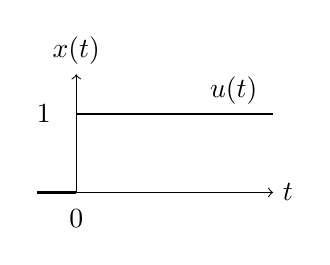
\begin{tikzpicture}
        \draw[->] (-0.5,0) -- (2.5,0) node[right] {$t$};
        \draw[->] (0,0) -- (0,1.5) node[above] {$x(t)$};

        \draw[thick] (-0.5,0) -- (0,0);
        \draw[thick] (0,1) -- (2.5,1);
        \draw[dashed] (0,0) -- (0,1);

        \node at (-0.2,1) [left] {$1$};
        \node at (0,-0.1) [below] {$0$};
        \node at (2,1) [above] {$u(t)$};
    \end{tikzpicture}\\
    図:単位ステップ関数
\end{center}
\end{minipage}

\vspace{2mm}

\end{tcolorbox}
% --------------- [3] --------------- 済
\begin{tcolorbox}[title={[3] 単位インパルス関数 \( x(t) = \delta(t) \)をラプラス変換せよ.}]

\vspace{4mm}

\quad 単位インパルス関数はディラックのデルタ関数ともよばれ,\( \delta(t) \) で記述される.\\
\quad \(h\)をゼロに近づけることで定義され,その面積では1である.

\vspace{-4mm}

\begin{minipage}[t]{0.6\linewidth}
    \begin{align*}
        &\quad \mathcal \int_{-\infty}^{\infty} \delta(t) dt = 1 \\[2mm]
        &\text{単位インパルス関数には次のような性質がある} \\[2mm]
        &\quad \mathcal \int_{-\infty}^{\infty} f(t)\delta(t-a) dt = f(a) \\[2mm]
        &\mathrm{Re}[s] > 0 \quad \text{の定義域において} \\[2mm]
        &\quad \mathcal{L}[\delta(t)] =\int_{0}^{\infty} e^{-st}\delta(t) dt =e^{-s・0} =  1 \\
    \end{align*}
\end{minipage}
\hfill
\begin{minipage}[t]{0.35\linewidth}
\vspace{10mm}
\begin{center}
    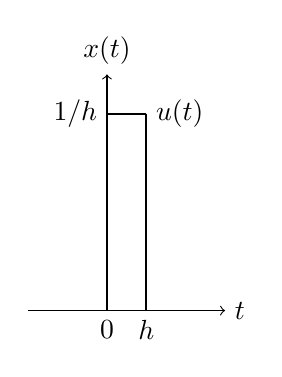
\begin{tikzpicture}
        \draw[->] (-1.0,0) -- (1.5,0) node[right] {$t$};
        \draw[->] (0,0) -- (0,3) node[above] {$x(t)$};

        \draw[thick] (0,2.5) -- (0.5,2.5);
        \draw[thick] (0.5,2.5) -- (0.5,0);

        \node at (0,2.5) [left] {$1/h$};
        \node at (0,0) [below] {$0$};
        \node at (0.5,0) [below] {$h$};
        \node at (0.5,2.5) [right] {$u(t)$};
    \end{tikzpicture}\\
    図:単位インパルス関数
\end{center}
\end{minipage}

\end{tcolorbox}
% --------------- [4] --------------- 済
\begin{tcolorbox}[title={[4] ランプ関数 \( x(t) = t \) をラプラス変換せよ.}]

\begin{minipage}{0.6\linewidth}
\begin{align*}
X(s) &= \int_0^{\infty} te^{-st} dt \\
&=\left[ t \left( - \frac{1}{s}e^{-st} \right) \right]_0^{\infty} - 
\int_0^{\infty} \left( -\frac{1}{s}e^{-st} \right) dt \\
&=0 + \frac{1}{s} \int_{0}^{\infty} e^{-st} \\
&=\frac{1}{s} \mathcal{L} \left[ 1 \right] \\
&=\frac{1}{s^2}
\end{align*}
\end{minipage}
\hfill
\begin{minipage}{0.35\linewidth}
\begin{center}
    \begin{tikzpicture}
        \draw[->] (-0.5,0) -- (2.5,0) node[right] {$t$};
        \draw[->] (0,0) -- (0,2.5) node[above] {$x(t)$};

        \draw[thick] (0,0) -- (2,2);
        \draw[dashed] (1,0) -- (1,1);
        \draw[dashed] (0,1) -- (1,1);

        \node at (0,1) [left] {$1$};
        \node at (0,0) [below] {$0$};
        \node at (1,0) [below] {$h$};
    \end{tikzpicture}\\
    図:ランプ関数
\end{center}
\end{minipage}

\end{tcolorbox}
% --------------- [5] --------------- 済
\begin{tcolorbox}[title={[5] 正弦波関数 \( x(t) = \sin(\omega t) \) をラプラス変換せよ.}]

\quad オイラーの等式より
\begin{align*}
\left\{
    \begin{aligned}
        e^{j \omega t} &= \cos(\omega t) + j \sin(\omega t) \\
        e^{-j \omega t} &= \cos(\omega t) - j \sin(\omega t)
    \end{aligned}
\right.
\end{align*}

\vspace{-2mm}

\begin{align*}
\mathcal{L} \left[ \sin(\omega t) \right] &=
\mathcal{L} \left[ \frac{1}{2j}\left( e^{j \omega t} - e^{-j \omega t} \right) \right] \\
&=\frac{1}{2j} \left( \frac{1}{s-j \omega} - \frac{1}{s + j \omega} \right) \\
&=\frac{1}{2j} \cdot \frac{2j\omega}{s^2 + \omega^2} \\
&=\frac{\omega}{s^2 + \omega^2}
\end{align*}

\end{tcolorbox}
% --------------- [6] --------------- 済
\begin{tcolorbox}[title={[6] 余弦波関数 \( x(t) = \cos(\omega t) \) をラプラス変換せよ.}]

\quad [5]と同様にして
\vspace{-2mm}
\begin{align*}
\mathcal{L} \left[ \cos(\omega t) \right] &=
\mathcal{L} \left[ \frac{1}{2}\left( e^{j \omega t} + e^{-j \omega t} \right) \right] \\
&=\frac{1}{2} \left( \frac{1}{s-j \omega} + \frac{1}{s + j \omega} \right) \\
&=\frac{1}{2} \cdot \frac{2s}{s^2 + \omega^2} \\
&=\frac{s}{s^2 + \omega^2}
\end{align*}

\end{tcolorbox}
% --------------- [7] --------------- 済
\begin{tcolorbox}[title={[7] \( e^{\lambda t} sin(\omega t) \) をラプラス変換せよ. }]

\quad ラプラス変換の第一移動定理(問題[8])

\[
    \mathcal{L} \left[ e^{at} f(t) \right] = F(s - a)
\]

と,正弦波のラプラス変換(問題[5])

\[
    \mathcal{L} \left[ sin(\omega t) \right] = \frac{\omega}{ s^2+ {\omega}^2} \quad \left( = X(s) \right)
\]

を考えれば,


\vspace{-3mm}
\begin{align*}
    \mathcal{L} \left[ e^{\lambda t} sin(\omega t) \right] &=
    X(s - \lambda) \\
    &=\frac{\omega}{ \left(s - \lambda \right)^2+ {\omega}^2}
\end{align*}

\vspace{2mm}
\vspace{2mm}
\end{tcolorbox}
% --------------- [8] --------------- 済
\begin{tcolorbox}[title={[8] 次の微分方程式をラプラス変換を用いて解け.
\[
    9 \frac{d^2 y(t)}{dt^2} + y(t) = 1 
\]
\quad ただし,初期値は,$y(0) = 0,\ y'(0) = 0$ とする.
}]

\quad まず,時間関数 \( y(t) \) の二階微分のラプラス変換は\( \mathcal{L} \left[ \frac{dy(t)}{dt} \right] = sY(s) - y(0) \)より,
    \vspace{-3mm}
    \begin{align*}
        \mathcal{L} \left[ \frac{d^2y(t)}{dt^2} \right] 
        &= s \mathcal{L} \left[ \frac{dy(t)}{dt} \right] - y'(0) \\
        &= s \left\{ sY(s) - y(0) \right\} - y'(0) \\
        &= s^2 Y(s) - s y(0) - y'(0)
    \end{align*}


\newpage

\quad 両辺にラプラス変換を施すと,

\vspace{-6mm}

\begin{align*}
    &\qquad 9 \mathcal{L} \left[ \frac{d^2 y(t)}{dt^2} \right] + \mathcal{L}[y(t)] = \mathcal{L}[1] \\
    &\Leftrightarrow \quad 9\left\{s^2 Y(s) - s y(0) - y'(0)\right\} + Y(s) = \frac{1}{s} \\
    &\Leftrightarrow \quad 9s^2 Y(s) + Y(s) = \frac{1}{s} \\
    &\Leftrightarrow \quad (9s^2 + 1) Y(s) = \frac{1}{s} \\
    &\Leftrightarrow \quad Y(s) = \frac{1}{s(9s^2 + 1)} \\
    &\Leftrightarrow \quad Y(s)= \frac{(\frac{1}{3})^2}{s(s^2 + \left( \frac{1}{3} \right)^2)} \\
    &\Leftrightarrow \quad Y(s)= \frac{\omega^2}{s(s^2 + \omega^2)} \quad \left[\because \omega = \frac{1}{3} \text{とおいた}\right]\\
    &\Leftrightarrow \quad Y(s)= \frac{\omega^2}{s(s + j \omega)(s - j \omega)} \\
    &\Leftrightarrow \quad Y(s)= \frac{1}{s} - \frac{\frac{1}{2}}{s + j \omega} - \frac{\frac{1}{2}}{s - j \omega} \quad \left[ \because ヘヴィサイドの展開定理 \right]
\end{align*}

\quad 両辺にラプラス逆変換を施すと,

\vspace{-6mm}

\begin{align*}
    &\qquad  \mathcal{L}^{-1} \left[ Y(s) \right]
    = \mathcal{L}^{-1} \left[ \frac{1}{s} \right] 
    - \frac{1}{2} \mathcal{L}^{-1} \left[\frac{1}{s + j \omega} \right]
    - \frac{1}{2} \mathcal{L}^{-1} \left[\frac{1}{s - j \omega} \right] \\
    &\Leftrightarrow \quad y(t) 
    = 1 - \frac{1}{2} e^{-j \omega t} - \frac{1}{2} e^{j \omega t} \\
    &\Leftrightarrow \quad y(t) 
    = 1 - \frac{1}{2} \left( e^{-j \omega t} + e^{j \omega t} \right) \\
    &\Leftrightarrow \quad y(t) 
    = 1 - cos{\omega t} \quad \left[ \because オイラーの等式 \right]\\
    &\Leftrightarrow \quad y(t) 
    = 1 - cos \left(\frac{t}{3}\right)
\end{align*}



\vspace{2mm}
\end{tcolorbox}
% --------------- [9] --------------- 済
\begin{tcolorbox}[title={[9] つぎの微分方程式をラプラス変換を用いて解け.
\[
\frac{d^2 x(t)}{dt^2} + 3 \frac{dx(t)}{dt} + 2x(t) = 4
\]
\quad ただし,初期条件は,$x(0)=1,\ x^{(1)}(0)=0$ とする. }]

\quad 両辺にラプラス変換を施すと,
\vspace{-3mm}
\begin{align*}
&\quad \mathcal{L} \left[ \frac{d^2 x(t)}{dt^2} + 3 \frac{dx(t)}{dt} + 2x(t) \right]
= \mathcal{L} \left[ 4 \right] \\
&\Leftrightarrow \left\{s^2 X(s) - sx(0)\right\} - x^{(1)}(0) + 3\left\{sX(s) - x(0) \right\} + 2X(s) = \frac{4}{s} \\
&\Leftrightarrow s^2 X(s) + 3sX(s) + 2X(s) = \frac{4}{s} + s + 3 \\
&\Leftrightarrow X(s) = \frac{\frac{4}{s} + s + 3}{s^2 + 3s + 2} = \frac{4 + s(s + 3)}{s(s + 1)(s + 2)} = \frac{s^2 + 3s + 4}{s(s + 1)(s + 2)} \\
&\Leftrightarrow X(s) = \frac{2}{s} - \frac{2}{s+1} + \frac{1}{s+2} \quad \left[ \because ヘヴィサイドの展開定理 \right]
\end{align*}

\quad 両辺にラプラス逆変換を施すと,
\vspace{-3mm}
\begin{align*}
&\quad \mathcal{L}^{-1} \left[ X(s) \right] 
= \mathcal{L}^{-1} \left[ \frac{2}{s} - \frac{2}{s+1} + \frac{1}{s+2} \right] \\
&\Leftrightarrow x(t) = 2 - 2e^{-t} + e^{-2t}
\end{align*}



\vspace{2mm}
\end{tcolorbox}
% --------------- [10] --------------- 済
\begin{tcolorbox}[title={[10] つぎの微分方程式をラプラス変換を用いて解け.\\
\[
\frac{dx(t)}{dt} + 3x(t) = sin{2t}
\]

\quad ただし,初期条件は,$x(0)=0$ とする. }]

\quad 両辺にラプラス変換を施すと,
\begin{align*}
    &\qquad \mathcal{L}\left[\frac{dx(t)}{dt} + 3\mathcal{L} x(t)\right] = \mathcal{L}\{\sin 2t\} \\
    &\Leftrightarrow sX(s) - x(0) + 3X(s) = \frac{2}{s^2 + 4} \\
    &\Leftrightarrow sX(s) + 3X(s) = \frac{2}{s^2 + 4} \\
    &\Leftrightarrow X(s) = \frac{2}{(s+3)(s^2 + 4)}  \\
    &\Leftrightarrow X(s)= \frac{2}{13} \left( \frac{1}{s+3} + \frac{3}{s^2 + 4} - \frac{s}{s^2 + 4} \right) 
    \quad \left[ \because ヘヴィサイドの展開定理 \right]
\end{align*}
    
\quad 両辺にラプラス逆変換を施すと,
\vspace{-3mm}
\begin{align*}
&\quad \mathcal{L}^{-1} \left[ X(s) \right] 
= \mathcal{L}^{-1} \left[ \frac{2}{13} \left( \frac{1}{s+3} + \frac{3}{s^2 + 4} - \frac{s}{s^2 + 4} \right) \right] \\
&\Leftrightarrow x(t) = \frac{1}{13} \left( 2e^{-3t} + 3\sin 2t - 2\cos 2t \right)
\end{align*}



\vspace{2mm}
\end{tcolorbox}
% --------------- [11] --------------- 済
\begin{tcolorbox}[title={[11] つぎの微分方程式をラプラス変換を用いて解け.\\
\[
\frac{d^2 x(t)}{dt^2} + 2\frac{dx(t)}{dt} + 2x(t) = 1 \\
\]

\quad ただし,初期条件は,$x(0)=1 , x^{(1)}(0)=1$ とする. }]

\quad 両辺にラプラス変換を施すと,
\begin{align*}
    &\qquad \mathcal{L}\left[ \frac{d^2 x(t)}{dt^2} + 2 \frac{dx(t)}{dt} + 2x(t) \right] = \mathcal{L}\{1\} \\
    &\Leftrightarrow \left\{s^2 X(s) - sx(0) - x^{(1)}(0) \right\} 
    + 2 \left\{ sX(s) - x(0) \right\} + 2X(s) 
    = \frac{1}{s} \\
    &\Leftrightarrow s^2 X(s) - 1 + 2sX(s) + 2X(s) = \frac{1}{s} \\
    &\Leftrightarrow s^2 X(s) + 2sX(s) + 2X(s) = s + 3 + \frac{1}{s} \\
    &\Leftrightarrow X(s) = \frac{s^2 + 3s + 1}{s(s^2 + 2s + 2)} \\
    &\Leftrightarrow X(s) = \left\{ \frac{\left(\frac{1}{2}\right)}{s} + \frac{\frac{1}{2}s+2}{s^2 + 2s + 2}  \right\} \\
    &\Leftrightarrow X(s) = \frac{1}{2} \left\{ \frac{1}{s} + \frac{\left(s+1\right)+3}{(s+1)^2 + 1^2}  \right\}
\end{align*}
\qquad 両辺にラプラス逆変換を施すと,
    \vspace{-3mm}
\begin{align*}
    \mathcal{L}^{-1}\{X(s)\} = \frac{1}{2} \left\{ 1 + e^{-t}(\cos t + 3 \sin t) \right\}
\end{align*}



\vspace{2mm}
\end{tcolorbox}

\newpage
% --------------- [12] ---------------

[12] (1)-(10)のラプラス変換$X(s)$にラプラス逆変換を施し,時間関数$x(t)$を求めよ.\\


% --------------- [12-1] --------------- 済
\begin{tcolorbox}[title={ [12] (1) \( X(s)=\frac{4}{s+5} \)}]
\quad 両辺にラプラス逆変換を施すと,
\vspace{-3mm}
\begin{align*}
    &\qquad \mathcal{L}^{-1} \left[ X(s) \right] 
    =\mathcal{L}^{-1} \left[ \frac{4}{s+5} \right] \\
    &\Leftrightarrow x(t) = 4 e^{-5t}
\end{align*}
\end{tcolorbox}
% --------------- [12-2] --------------- 済
\begin{tcolorbox}[title={ [12] (2) \( X(s)=\frac{ s + 7 }{ s^2 + 2s + 5} \)}]
\vspace{-3mm}
\begin{align*}
    &\qquad X(s) =\frac{ s + 7 }{ s^2 + 2s + 5}  \\
    &\Leftrightarrow X(s) =\frac{ (s + 1) + 6 }{ ( s + 1 )^2+ 2^2} \\
    &\Leftrightarrow X(s) 
    = \frac{ (s + 1) }{ ( s + 1 )^2+ 2^2}
    + \frac{ 6 }{ ( s + 1 )^2+ 2^2} 
\end{align*}

\quad 両辺にラプラス逆変換を施すと,
\vspace{-3mm}
\begin{align*}
    &\qquad \mathcal{L}^{-1} \left[ X(s) \right] 
    =\mathcal{L}^{-1} \left[ \frac{ (s + 1) }{ ( s + 1 )^2+ 2^2} \right]
    +\mathcal{L}^{-1} \left[ \frac{ 6  }{ ( s + 1 )^2+ 2^2} \right] \\
    &\Leftrightarrow x(t) = e^{-t} cos(2t) +3 e^{-t} sin(2t)
\end{align*}
\end{tcolorbox}
% --------------- [12-3] --------------- 済
\begin{tcolorbox}[title={ [12] (3) \( X(s)=\frac{ 2 }{ s^2 + s } \)}]
\vspace{-3mm}
\begin{align*}
    &\qquad X(s) =\frac{ 2 }{ s^2 + s }  \\
    &\Leftrightarrow X(s) =\frac{ 2 }{ s(s+1) }  \\
    &\Leftrightarrow X(s) 
    = \frac{2}{s}
    + \frac{-2}{s + 1} 
    \quad [\because ヘヴィサイドの展開定理]
\end{align*}

\quad 両辺にラプラス逆変換を施すと,
\vspace{-3mm}
\begin{align*}
    &\qquad \mathcal{L}^{-1} \left[ X(s) \right] 
    =\mathcal{L}^{-1} \left[ \frac{2}{s} \right]
    -\mathcal{L}^{-1} \left[ \frac{2}{s + 1} \right] \\
    &\Leftrightarrow x(t) = 2 - 2 e^{-t}
\end{align*}\end{tcolorbox}
% --------------- [12-4] --------------- 済
\begin{tcolorbox}[title={ [12] (4) \( X(s)=\frac{ s + 1 }{ s ( s^2 + 4s + 8 ) } \)}]
\vspace{-3mm}
\begin{align*}
    &\qquad X(s) =\frac{ s + 1 }{ s ( s^2 + 4s + 8 ) }  \\
    &\Leftrightarrow X(s) 
    = \frac{ \frac{1}{8} }{s}
    +\frac{ -\frac{1}{8}(s-4) }{ s^2 + 4s + 8 } 
    \quad [\because ヘヴィサイドの展開定理]\\
    &\Leftrightarrow X(s) 
    =\frac{1}{8s}
    -\frac{ (s+2)-6}{8\left\{(s+2)^2 + 4 \right\}}
\end{align*}

\quad 両辺にラプラス逆変換を施すと,
\vspace{-3mm}
\begin{align*}
    &\qquad \mathcal{L}^{-1} \left[ X(s) \right] 
    =\mathcal{L}^{-1} \left[ \frac{1}{8s} \right]
    -\mathcal{L}^{-1} \left[ \frac{ (s+2)-6}{8\left\{(s+2)^2 + 4 \right\}} \right] \\
    &\Leftrightarrow x(t) = \frac{1}{8} - \frac{1}{8}e^{-2t}(cos(2t)-3sin(2t))
\end{align*}
\end{tcolorbox}
% --------------- [12-5] --------------- 済
\begin{tcolorbox}[title={ [12] (5) \( X(s)=\frac{ 1 }{ s^3 + 11 s^2+ 40s + 48 } \) }]
\vspace{-3mm}
\begin{align*}
    &\qquad X(s) =\frac{ 1 }{ s^3 + 11 s^2+ 40s + 48 }  \\
    &\Leftrightarrow X(s) =\frac{ 1 }{ (s+3)(s+4)^2 }  \\
    &\Leftrightarrow X(s) 
    = \frac{1}{s+3}
    + \frac{-1}{s + 4}
    + \frac{-1}{(s + 4)^2}
    \quad [\because ヘヴィサイドの展開定理]
\end{align*}

\quad 両辺にラプラス逆変換を施すと,
\vspace{-3mm}
\begin{align*}
    &\qquad \mathcal{L}^{-1} \left[ X(s) \right] 
    =\mathcal{L}^{-1} \left[ \frac{1}{s+3} \right]
    +\mathcal{L}^{-1} \left[ \frac{-1}{s + 4} \right]
    +\mathcal{L}^{-1} \left[ \frac{-1}{(s + 4)^2} \right] \\
    &\Leftrightarrow x(t) = e^{-3t} - e^{-4t} - te^{-4t}
\end{align*}
\end{tcolorbox}
% --------------- [12-6] --------------- 済
\begin{tcolorbox}[title={ [12] (6) \( X(s)=\frac{ 2 }{ ( s + 1 ) ( s + 3 ) } \)}]
\vspace{-3mm}
\begin{align*}
    &\qquad X(s) =\frac{ 2 }{ ( s + 1 ) ( s + 3 ) }  \\
    &\Leftrightarrow X(s) 
    = \frac{1}{s + 1}
    + \frac{-1}{s + 3} 
    \quad [\because ヘヴィサイドの展開定理]
\end{align*}

\quad 両辺にラプラス逆変換を施すと,
\vspace{-3mm}
\begin{align*}
    &\qquad \mathcal{L}^{-1} \left[ X(s) \right] 
    =\mathcal{L}^{-1} \left[ \frac{1}{s + 1} \right]
    +\mathcal{L}^{-1} \left[ \frac{-1}{s + 3} \right] \\
    &\Leftrightarrow x(t) = e^{-t} - e^{-3t}
\end{align*}
\end{tcolorbox}
% --------------- [12-7] --------------- 済
\begin{tcolorbox}[title={ [12] (7) \( X(s)=\frac{ 3 }{ s ( s + 2)^2 } \)}]
\vspace{-3mm}
\begin{align*}
    &\qquad X(s) =\frac{ 3 }{ s ( s + 2)^2 }  \\
    &\Leftrightarrow X(s) 
    = \frac{(\frac{3}{4})}{s}
    + \frac{(-\frac{3}{4})}{s + 2} 
    + \frac{(-\frac{3}{2})}{(s + 2)^2} 
\end{align*}

\quad 両辺にラプラス逆変換を施すと,
\vspace{-3mm}
\begin{align*}
    &\qquad \mathcal{L}^{-1} \left[ X(s) \right] 
    = \mathcal{L}^{-1} \left[\frac{(\frac{3}{4})}{s} \right]
    + \mathcal{L}^{-1} \left[ \frac{(-\frac{3}{4})}{s + 2} \right]
    + \mathcal{L}^{-1} \left[\frac{(-\frac{3}{2})}{(s + 2)^2}\right]\\
    &\Leftrightarrow x(t) = \frac{3}{4}-\frac{3}{4}e^{-2t}-\frac{3}{2}te^{-2t}
\end{align*}
\end{tcolorbox}
% --------------- [12-8] --------------- 済
\begin{tcolorbox}[title={ [12] (8) \( X(s)=\frac{ 1 }{ s ( s + 2 ) ( s + 3 )^2 } \) }]
\vspace{-3mm}
\begin{align*}
    &\qquad X(s) =\frac{ 1 }{ s ( s + 2 ) ( s + 3 )^2 }  \\
    &\Leftrightarrow X(s) 
    = \frac{\frac{1}{18}}{s}
    + \frac{(-\frac{1}{2})}{s + 2} 
    + \frac{\frac{1}{3}}{(s + 3)^2} 
    + \frac{\frac{4}{9}}{s + 3} 
\end{align*}

\quad 両辺にラプラス逆変換を施すと,
\vspace{-3mm}
\begin{align*}
    &\qquad \mathcal{L}^{-1} \left[ X(s) \right] 
    =\mathcal{L}^{-1} \left[ \frac{\frac{1}{18}}{s} \right]
    + \mathcal{L}^{-1} \left[ \frac{(-\frac{1}{2})}{s + 2} \right]
    + \mathcal{L}^{-1} \left[ \frac{\frac{1}{3}}{(s + 3)^2} \right]
    + \mathcal{L}^{-1} \left[ \frac{\frac{4}{9}}{s + 3} \right] \\
    &\Leftrightarrow x(t) = \frac{1}{18} - \frac{1}{2}e^{-2t} + \frac{1}{3}e^{-3t} +\frac{4}{9}e^{-3t}\\
    &\Leftrightarrow x(t) =\frac{1}{18} \left(1 - 9e^{-2t} + 8e^{-3t} +6te^{-3t} \right)
\end{align*}
\end{tcolorbox}
% --------------- [12-9] --------------- 済
\begin{tcolorbox}[title={ [12] (9) \( X(s)=\frac{ s + 2 }{s^3 ( s - 1 )^2 } \) }]
\vspace{-3mm}
\begin{align*}
    &\qquad X(s) =\frac{ s + 2 }{ ( s - 1 )^2 s^3 }  \\
    &\Leftrightarrow X(s) 
    = \frac{2}{s^3}
    + \frac{5}{s^2} 
    + \frac{8}{s}
    + \frac{3}{(s - 1)^2}
    + \frac{-8}{s - 1}
\end{align*}

\quad 両辺にラプラス逆変換を施すと,
\vspace{-3mm}
\begin{align*}
    &\qquad \mathcal{L}^{-1} \left[ X(s) \right] 
    =\mathcal{L}^{-1} \left[
        \frac{2}{s^3}
    + \frac{5}{s^2} 
    + \frac{8}{s}
    + \frac{3}{(s - 1)^2}
    + \frac{-8}{s - 1} \right] \\
    &\Leftrightarrow x(t) = \left(t^2+5t+8\right) + \left(3t-8\right) e^{t}
\end{align*}
\end{tcolorbox}
% --------------- [12-10] --------------- 済
\begin{tcolorbox}[title={ [12] (10) \( X(s)=\frac{ 1 }{ ( s^2 + 1 ) ( s^2 + 4 ) } \) }]
\vspace{-3mm}
\begin{align*}
    &\qquad X(s) =\frac{ 1 }{ ( s^2 + 1 ) ( s^2 + 4 ) } \\
    &\Leftrightarrow X(s) 
    = \frac{ \frac{1}{3} }{ ( s^2 + 1 ) }
    + \frac{ -\frac{1}{3} }{ ( s^2 + 4 ) }
\end{align*}

\quad 両辺にラプラス逆変換を施すと,
\vspace{-3mm}
\begin{align*}
    &\qquad \mathcal{L}^{-1} \left[ X(s) \right] 
    =\mathcal{L}^{-1} \left[ \frac{ \frac{1}{3} }{ ( s^2 + 1 ) } \right]
    +\mathcal{L}^{-1} \left[ \frac{- \frac{1}{3} }{ ( s^2 + 4 ) } \right] \\
    &\Leftrightarrow x(t) = \frac{1}{3}sin t -\frac{1}{6}sin 2t
\end{align*}

\end{tcolorbox}
% --------------- [13] --------------- 済
\begin{tcolorbox}[title={[13] つぎの微分方程式をラプラス変換を用いて解け.\\
\[
\frac{d^2y(t)}{dt^2} + y(t) = 0
\]

\quad ただし,初期条件は,\(y(0)=A, y^{(1)}(0)=B\) とする. }]

\quad 両辺にラプラス変換を施すと,
\vspace{-3mm}
\begin{align*}
    &\qquad \mathcal{L}\left[ \frac{d^2y(t)}{dt^2} + y(t) \right] = 0 \\
    &\Leftrightarrow \left\{ s^2 Y(s) - sy(0) - y^{(1)}(0) \right\} + Y(s) = 0  \\
    &\Leftrightarrow s^2 Y(s) - A s - B + Y(s) = 0  \\
    &\Leftrightarrow Y(s) = \frac{As + B}{ s^2 + 1}  \\
    &\Leftrightarrow Y(s) = \frac{As}{ s^2 + 1} + \frac{B}{ s^2 + 1} 
\end{align*}
    
\quad 両辺にラプラス逆変換を施すと,
\vspace{-3mm}
\begin{align*}
&\qquad \mathcal{L}^{-1} \left[ Y(s) \right] 
= \mathcal{L}^{-1} \left[ \frac{As}{ s^2 + 1} + \frac{B}{ s^2 + 1}  \right] \\
&\Leftrightarrow y(t) = A cos{t} + B sin{t}
\end{align*}
\end{tcolorbox}
% --------------- [14] --------------- 済
\begin{tcolorbox}[title={[14] つぎの微分方程式をラプラス変換を用いて解け.\\
\[
\frac{d^2y(t)}{dt^2} -( a + b )\frac{dy(t)}{dt} + a b y(t) = 0
\]

\quad ただし,初期条件は,\(y(0)=1, y^{(1)}(0)=0\) とする.}]

\quad 両辺にラプラス変換を施すと,
        \vspace{-3mm}
        \begin{align*}
            &\qquad \mathcal{L}\left[ \frac{d^2y(t)}{dt^2} - ( a + b )\frac{dy(t)}{dt} + a b y(t) \right] = 0 \\
            &\Leftrightarrow \left\{ s^2 Y(s) - sy(0) - y^{(1)}(0) \right\}
            - (a+b)\left\{ sY(s) - y(0) \right\}
            + abY(s) = 0  \\
            &\Leftrightarrow \left\{ s^2 - (a + b) s + ab\right\} Y(s) - s + ( a + b )= 0  \\
            &\Leftrightarrow Y(s) = \frac{s - (a + b)}{ s^2 - (a + b) s + ab }  \\
            &\Leftrightarrow Y(s) =  \frac{s - (a + b)}{ (s - a)(s - b) }  \\
            &\Leftrightarrow Y(s) =  \frac{- \frac{b}{a-b}}{ (s - a) } + \frac{ \frac{a}{a-b}}{ (s - b) }
        \end{align*}
            
        \quad 両辺にラプラス逆変換を施すと,
        \vspace{-3mm}
        \begin{align*}
        &\qquad \mathcal{L}^{-1} \left[ Y(s) \right] 
        = \mathcal{L}^{-1} \left[ \frac{- \frac{b}{a-b}}{ (s - a) } + \frac{ \frac{a}{a-b}}{ (s - b) }  \right] \\
        &\Leftrightarrow y(t) = - \frac{b}{a-b}e^{at} + \frac{a}{a-b}e^{bt}
        \end{align*}
    \end{tcolorbox}
% --------------- [15] --------------- 済
\begin{tcolorbox}[title={[15] つぎの微分方程式をラプラス変換を用いて解け.\\
\[
\frac{d^2y(t)}{dt^2} - \frac{dy(t)}{dt} - 12 y(t) = 2
\]

\quad ただし,初期条件は,\(y(0)=1, y^{(1)}(0)=0\) とする.}]

\quad 両辺にラプラス変換を施すと,
    \vspace{-3mm}
    \begin{align*}
        &\qquad \mathcal{L}\left[ \frac{d^2y(t)}{dt^2} - \frac{dy(t)}{dt} - 12 y(t) \right] 
        = \mathcal{L} \left[ 2 \right] \\
        &\Leftrightarrow \left\{ s^2 Y(s) - sy(0) - y^{(1)}(0) \right\}
        - \left\{ sY(s) - y(0) \right\}
        - 12 Y(s) = \frac{2}{s}  \\
        &\Leftrightarrow \left\{ s^2 - s - 12 \right\} Y(s) - s + 1= \frac{2}{s}  \\
        &\Leftrightarrow Y(s) = \frac{s^2 - s + 2}{s(s^2 - s - 12)}  \\
        &\Leftrightarrow Y(s) =  \frac{s^2 - s + 2}{ s (s + 3)(s - 4) }  \\
        &\Leftrightarrow Y(s) =  \frac{- \frac{1}{6}}{ s } + \frac{  \frac{2}{3} }{ s + 3 } + \frac{  \frac{1}{2} }{ s - 4 } 
        \quad \left[\because ヘヴィサイドの展開定理 \right]
    \end{align*}
        
    \quad 両辺にラプラス逆変換を施すと,
    \vspace{-3mm}
    \begin{align*}
    &\qquad \mathcal{L}^{-1} \left[ Y(s) \right] 
    = \mathcal{L}^{-1} \left[ \frac{- \frac{1}{6}}{ s } + \frac{  \frac{2}{3} }{ s + 3 } + \frac{  \frac{1}{2} }{ s - 4 }  \right] \\
    &\Leftrightarrow y(t) = - \frac{1}{6} + \frac{2}{3}e^{-3t} + \frac{1}{2}e^{4t}
    \end{align*}
\end{tcolorbox}
% --------------- [16] --------------- 済
\begin{tcolorbox}[title={[16] つぎの微分方程式をラプラス変換を用いて解け.\\
\[
\frac{d^2y(t)}{dt^2} + 4 y(t) = sin(t)
\]

\quad ただし,初期条件は,\(y(0)=0, y^{(1)}(0)=0\) とする. }]


    \quad 両辺にラプラス変換を施すと,
    \vspace{-3mm}
    \begin{align*}
        &\qquad \mathcal{L}\left[ \frac{d^2y(t)}{dt^2} + 4 y(t) \right] 
        = \mathcal{L} \left[ sin(t) \right] \\
        &\Leftrightarrow \left\{ s^2 Y(s) - sy(0) - y^{(1)}(0) \right\}
        + 4 Y(s) = \frac{1}{s^2 + 1}  \\
        &\Leftrightarrow \left\{ s^2 + 4 \right\} Y(s) = \frac{1}{s^2 + 1}  \\
        &\Leftrightarrow Y(s) = \frac{1}{(s^2+1)(s^2+4)}  \\
        &\Leftrightarrow Y(s) = \frac{ \frac{1}{3} }{s^2+1} - \frac{ \frac{1}{3} }{s^2+4} 
        \quad \left[\because ヘヴィサイドの展開定理 \right]
    \end{align*}
        
    \quad 両辺にラプラス逆変換を施すと,
    \vspace{-3mm}
    \begin{align*}
    &\qquad \mathcal{L}^{-1} \left[ Y(s) \right] 
    = \mathcal{L}^{-1} \left[  \frac{ \frac{1}{3} }{s^2+1} - \frac{ \frac{1}{3} }{s^2+4}   \right] \\
    &\Leftrightarrow y(t) = \frac{1}{3}sin(t) - \frac{1}{6}sin(2t)
    \end{align*}
\end{tcolorbox}
\end{document}